\section{Introduction}

  \par Bike shares are riding a wave of popularity in the intermodal transit planning community. Through bike sharing systems in a city, people are able to rent a bike from a one location and return it to a different place on an as-needed basis. The number of bike share systems, defined as publicly-available systems with at least 10 stations and 100 bikes, has steadily increased year-over-year, from four systems in 2010 to 55 systems in 2016 across U.S, with over 42,000 bikes available in cities of all sizes\cite{us}. In addition, 80\% of systems that have been in operation for more than a year have expanded since they launched. The number of bikes in the nation also increased substantially, up 30\%, as existing large systems have continued to grow. Figure \ref{fig_intro} shows the bike share growth in the US from 2010 to 2016\footnote{Figure taken from https://nacto.org/bike-share-statistics-2016/, December 02, 2017}.
  \par The growth of bike share shows no signs of stopping. A number of U.S. cities, such as Detroit, New Haven, and New Orleans, have either selected vendors or are planning to launch systems, and many existing systems are also rolling out major expansions: New York's Citi Bike Program \cite{bike} is adding another 2,000 bikes, for a total of 12,000; Houston is more than tripling in size to over 100 stations; and the San Francisco Bay Area is expanding from a 700 to a 7,000 bike system\cite{spread}. Here in our assignment, we conduct a case study based on the bike sharing data on the Citi Bike Share System in New York City in order to predict the duration for a user in one bike trip at a certain time. We try to forecast the duration of a share-bike trip to help improve and expand the bike sharing system in NYC. Predicting duration of a bike ride can also help users to make wise decisions on hailing a cab or riding a bike, for example. 

  \begin{figure}[h]
  \centering
  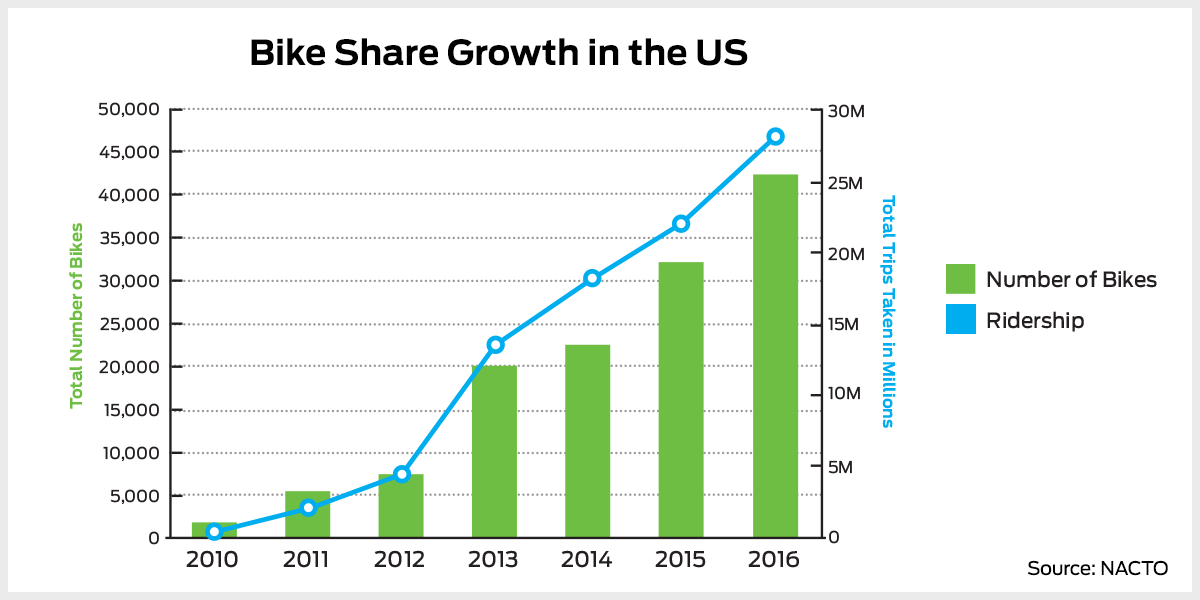
\includegraphics[width=0.4\textwidth]{intro}
  \caption{Bike Share Growth in the US}
  \label{fig_intro}
  \end{figure}
  % h means put it here
  % * means not in two columns

  \par In this project, we obtained the primary dataset provided by Citibike System Data. The data generated by these bike share systems are consisted of duration of travel, start time and date, stop time and date, start station name, stop station name, station ID, station latitude and lonitude, bike ID, user type(Customer = 24-hour pass or 3-day pass user; Subscriber = Annual Member), user gender and user's year of birth. Given adequate data from Jul 2013 to Sep 2017, we used data in 2016 year round. In our analysis, we attempt to evaluate the importance of different features and extract the non-trivial ones to create a prediction model for this problem. We then compare performances of different models and discuss their effectiveness and shortcomings. In this assignment, We mainly use the method of multiple linear regression analysis, Random Forest and XGBoost to forecast the bike share trip duration in New York City. An ensemble of Random Forest and XGBoost is also applied in this report. We evaluate these models based on the Fraction of Variance Unexplained (FVU). 

\section{Data}
\subsection{Dataset Variables}
  \par We obtain the data from the data system of Citi Bike, which is the national largest bike share program, with 10,000 bikes and 600 stations across Manhattan, Brooklyn, Queens and Jersey City\cite{bike}. It consists of data from the program's launch date, from 07/2013 to 09/2017. The dataset provided information\footnote{Customer = 24-hour pass or 3-day pass user; Subscriber = Annual Member}\footnote{0=unknown; 1=male; 2=female} is as shown in Table \ref{tab_1}. 
	\begin{center}
	\begin{table}[h!]
	\caption{Dataset Variable and Type}
	\label{tab_1}
	\begin{tabular}{ |c|c| } 
	 \hline
	 Variate & Format \\ 
	 \hline
	 Trip Duration & in seconds format \\ 
	 \hline
	 Start Time and Date & Timestamp\\ 
	 \hline
	 Stop Time and Date & Timestamp\\
	 \hline
	 Start Station Name & String\\
	 \hline
	 End Station Name & String\\
	 \hline
	 Station ID & Number\\
	 \hline
	 Station Lat/Long & Number\\
	 \hline
	 Bike ID & Number\\
	 \hline
	 User Type & Customer or Subscriber  \\
	 \hline
	 Gender & Number  \\
	 \hline
	 Year of Birth & Number\\
	 \hline
	\end{tabular}
	\end{table}
	\end{center}	
\subsection{Data Cleaning}
	\par Basically, there were [XXXX] bike stations and total number of rides in dataset is [XXXXX]. Total number of customers' rides is [XXXXX] and subscribers' rides is [XXXX]. 
	\par From a preliminary analysis on these data, we need to detect and deal with some abnormal data. For some cases too short duration or even zero or negative is deleted; cases that takes too long duration in a trip (> 1 million seconds, roughly around a month) are also removed; for some cases the users' information are missing, age and sex, for example; for some the ratio of distance by duration is unreasonably high (30 mile/hour) or low (1 mile/hour). A lower bound (2.2369 mile/hour) and an upper bound (19.0137 mile/hour) is used in this analysis to protect our models from being skewed by extremities and make them immune to outliers, which is a reasonable range from walking to driving\cite{zheng}.
	\par After all these data cleaning, we randomly choose 30k trips from each month in 2016, which creates a dataset with a size of 360k in total. And we split it into three sets: training, validation and test, each with 120,000 rides.
\subsection{Exploratory Analysis}
	\par To understand [Here we need a picture to show the overall distribution of bike duration. --> each year][show the time period that the dataset cover...]
	[Different Pictures...]
	[EDA]
	\subsubsection{prevelance}
	\par Fig.X illustrates an increase in the number of trips starting from 2014, when the citi bike program just launched to 2017. This shows that more and more people start to [PIC!!!!!!]



\section{Predictive Task}
Based on the given dataset, what we want to do is to predict a single trip duration in the Citi Bike Share System in New York City.

\subsection{Evaluation Method}
We evaluate the performance of different models on the basis of the fraction of variance unexplained (FVU). FVU is calculated as:
\[FVU(f) =1-R^2 = \frac{MSE(f)}{Var(y)}\]
\par FVU is suitable for our problem because FVU in statistics, is the fraction of variance of the regressand (dependent variable) Y which cannot be explained, i.e., which is not correctly predicted, by the explanatory variables X. When trying to predict Y, the most naive regression function that we can think of is the constant function predicting the mean of Y, i.e., $f(x_{i})=\bar{y}$. It follows that the MSE of this function equals the variance of Y and the FVU then reaches its maximum value of 1. So if the explanatory variables X tell us nothing about Y, $FVU(f)=1$. But as prediction gets better, MSE can then be reduced and ideally the best modle will have $FVU(f) = 0$. 

\subsection{Data Preprocessing}
\par In this dataset, 30k observations is randomly extracted from data in each month in 2016. And this aggregated dataset now contains 360k observations and is well distributed in all year round. It is then shuffled and divided into three splits, individually 1/3 for training, validation and test. Each training sample consists of 15 entries -- the first 11 contains the basic information for a certain bike trip. In addition, there are also 4 entries that represent the rider's information. To make a better use of these training samples, we preprocess and convert them into a more intuitive form as described below.
\begin{enumerate}
	\item Day of month:
	\par From the given timestamp of the start date and end date we can easily compute the day of the month, and we use it as 31 features to represent different days in a month. 
	\item Day of week:
	\par Using the timestamp provided in our dataset, by using one-hot encoding, we construct 7 features to represent different days in a week in order to provide more explantion on weekdays and weekends.
	\item Year:
	\par As we focused mainly on data in 2016, so the year feature here is set all 2016, and in later discussion be left behind.
	\item Month:
	\par With the same technique, we use 12 features to represent the months from January to December.
	\item Hours:
	\par Given the specific start time and stop time, by one-hot encoding we can use 24 features to represent the 24 hours in a day.
	\item Minutes:
	\par From the timestamp value present in the data set, we divide 0$\sim$60 minutes into four features, each of them covers a range in 15 minutes.
	\item Distance:
	\par Given latitude and longitude of the start location and stop location, we can calculate 
	In order to represent the latitude and longitude information of the start and end station in some useful forms, we consider several different ways, such as mapping them into zip code and use one-hot encoding to represent them into categorical features. Due to the largeness of our data set, it takes too long to convert each pair of latitude and longitude into a zip code representation. We choose to use the distance between the start station and end station as the feature. The  conversion is simply by using the vincenty distance of the Geopy library in Python\cite{geopy}. 
	\item Gender:
	\par In the orginal dataset, 1 for males and 2 for females. After processing, we convert it into a boolean feature, 1 for females and 0 for males.
	\item Age:
	\par In order to represent the age in a useful form, we set 30 year-old as a watershed and use two categories to represent it. If the given age is smaller than or equal to 30, we set the negative value of given age to the first category and 0 to the second category. If the given age is greater than 30, we set 30 to the first category and the difference between the given age and 30 to the second category. For example, if the given age is 15, then we set -15 to the first category and 0 as the second. If the given age is 40, then we set 30 to the first category and 10 to the second. The intuition to represent the feature age in this way is that we consider the age 30 and below is negatively related to the duration of the ride, which means that the closer to the 30, the shorter duration it takes. And we consider the age above 30 is positively related to the duration of the ride, which means that the further to the 30, the longer duration it takes.  

\end{enumerate}


\subsection{Features Selection}
The previous exploratory analysis on different features illustrated a few imporatant features that we should include. We firstly incorporated the latitude and longitude of the start and end station, month, week, hour, minutes, gender and age as our feature vectors. To analyze the importance of each feature, we remove each of these features from our feature set to see how the performance changes. Fig.X shows the importance of each chosen features. [PIC!!!!!] \par

[Time this part... ] \par
When we consider if selecting the day or week as one of the features and if adding time into the feature vector, there are different opinions in our group, so we draw a bar graph (Fig. \ref{fig_date}) to compare four cases: week, week and time, day, day and time. We add one of these combinations into our feature set each time and run our linear regression model to see which one works best. As shown in the graph, by adding the features week and time, the performance is the best. 

Most improtant features observed for our prediction task are distance.....

  \begin{figure}[h!]
  \centering
  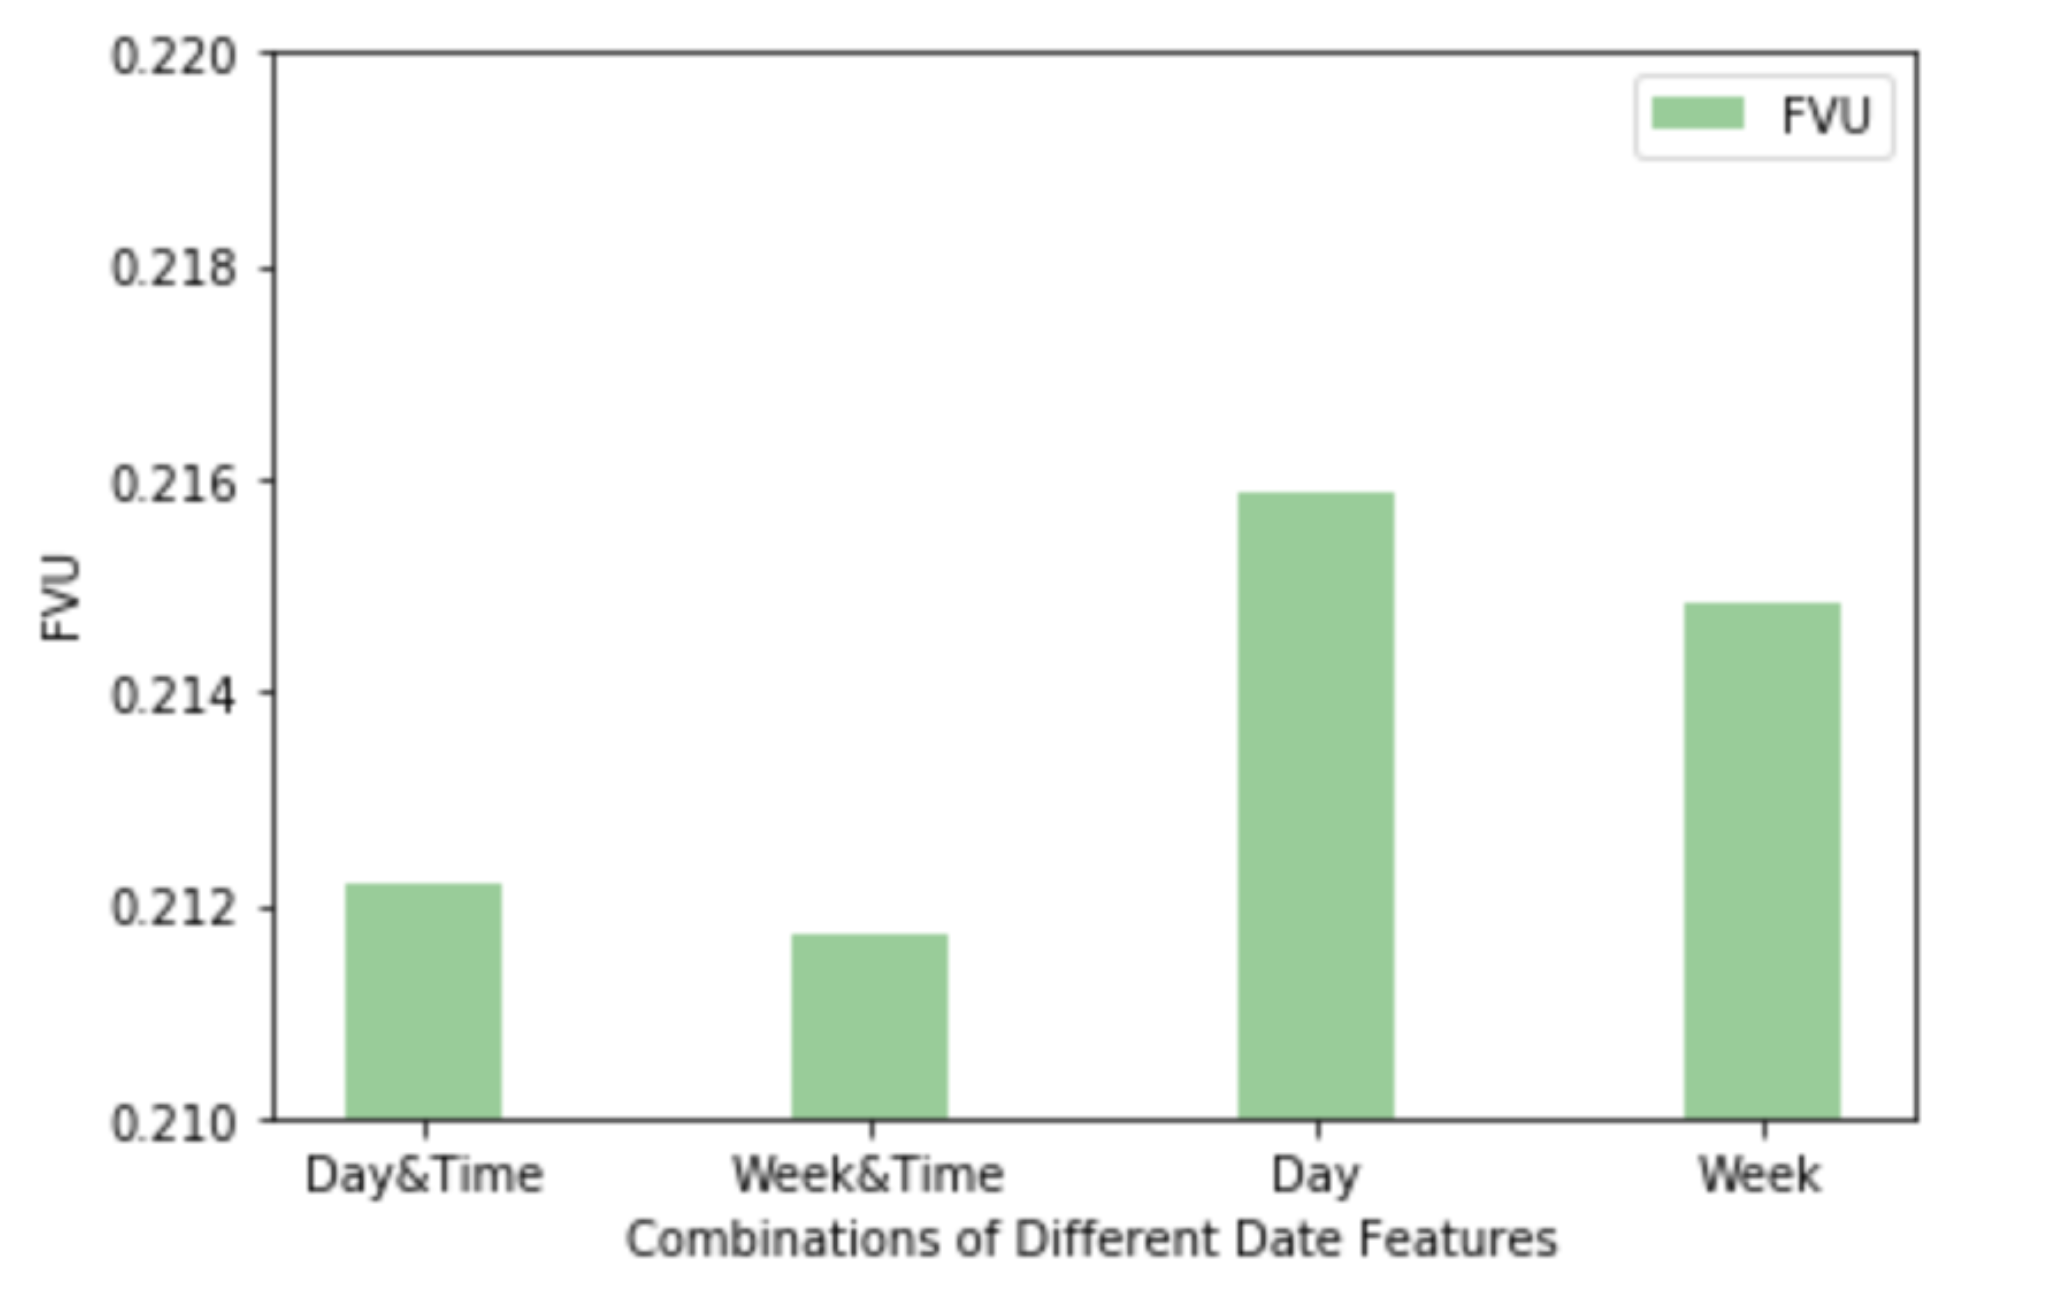
\includegraphics[width=0.4\textwidth]{ink}
  \caption{Date and Time Feature Selection}
  \label{fig_date}
  \end{figure}



\section{Models and Methodology}

\section{Literature}
\subsection{Relevant Dataset}
\par Our dataset is provided by New York Citi Bike Share System and most of the bike share system provide opening dataset in similar formula to public. Similar dataset can also be visited and gained through Hubway Bike Share System in Boston, MA\footnote{Hubway Bike Share:
\url{http://www.cambridgema.gov/CDD/Transportation/gettingaroundcambridge/bikeshare}}; DecoBike in Miami, FL\footnote{Deco Bike, Citi Bike:
\url{http://citibikemiami.com}}; Relay Bike Share System in Atlanta, GA\footnote{Relay Bike Share:
\url{http://relaybikeshare.com/system-data/}}; Reddy Bike Share System in Buffalo, NY\footnote{Relay Bike Share:
\url{https://reddybikeshare.socialbicycles.com}}; Divvy Bike Share System in Chicago, IL\footnote{Divvy Bike Share:
\url{https://www.divvybikes.com}}; Capital Bike Share System in Washington, DC\footnote{Relay Bike Share:
\url{https://www.capitalbikeshare.com/system-data}},etc. These systems generate a great deal of data relating to various ride details, including trip duration, start and end location, etc.
\par The dataset we used here is of great importance for us to study public transporation and city mobility. Leveraging the historical data provided can benefit us to providing more accurate prediction for bike trip duration at a time.
\subsection{Related Work}
\par Many previous research and investigation have been conducted in bike trip prediction. But most of them are forcasting the share bike demand at a certain time or at a certain place. Also, there has been a share bike demand prediction Competition running on Kaggle three years ago. But few of relevant projects are delved into bike trip duration prediction as what we did in this project.
\par For those who are predicting the share bike demand, some techniques and key features that they have used and worth mentioning are as follows:

\subsubsection{Geographic and Distance Information}
Javier etc.\cite{gu} develops a rapid response ridership forecast model, based on the combined use of Geographic Information Systems (GIS), distance-decay functions and multiple regression models. Analyses carried out show that weighting the variables according to the distance-decay functions provides systematically better results. The choice of distance threshold also significantly improves outcomes. Osvaldo etc. \cite{car} develops models based on GIS and proves its considerable advantages over the traditional four-step model, including simplicity of use, easy interpretation of results, immediate response and low cost. This study also uses geographically weighted regression (GWR) to deal with the staion prediction problem. Patrick etc.\cite{vogel} refrains from building a spatial model to assess the bike share repositioning services.

\subsubsection{Bike Docking Station Locations}
\par Yexin Li etc.\cite{Li} proposed a bipartite prediction algorithm based on hierarchical clustering to cluster bike stations into groups and therefore get different levels of hierarchical bike stations.

\subsubsection{User Subscription Plans and User Habits}
Elliot etc.\cite{fish} investigates several significant predictors of membership includingreactions to mandatory helmet legislation, riding activity over the previous month, and the degree to which convenience motivated private bike riding. These results provide insight as to the relative influence of various factors impacting on bike share membership in Australia. The findings may assist bike share operators to maximize membership potential and help achieve the primary goal of bike share – to increase the sustainability of the transport system.

\subsubsection{Time Series Data}
To predict the demand of bikes, a multi-similarity-based interference model based on gradient boosting regression tree is proposed to predict the rent proportion across clusters and the inter-cluster transition, based on which the number of bikes rent from/returned to each cluster can be easily inferred\cite{Li}. 

\subsection{Analysis on this task}
From the aboved analysis, we can see most of the prediction task are trying to solve the re-allocation problem or the arrangement of the bike docking station problem. So they pay more attention on the specific bike docking stations and try to deeply understand users' habits. Also, a majority of these investigations are made to predict the bike demand for an entire area and that is why they care more about geographic features. However, our predictive task is different from above mentioned work because we are trying to predict the duration of each bike trip. So we convert the specific location information such as longtitude and latitude to a more concrete distance feature during a trip. Also, the user's habit and subscription would be helpful in our prediction and we also included sexuality, age and other user information in our predcition models. 

\section{Results and Conclusions}

\subsection{Results}
FVU values with different models in this duration prediction task calculated with different models we built are as follows:

[Table or Picture !!!]

From comparison of different models we can get a lowest FVU of [XXXX] with XGBoosting Regressor as a bike trip duration prediction model, which can helps provide efficient and accurate duration prediction for each bike trip.

\subsection{Conclusions}

\subsection{Future Work}

% \end{document}  % This is where a 'short' article might terminate

